%  公立はこだて未来大学 卒業論文 テンプレート ver1.50
% (c) Junichi Akita (akita@fun.ac.jp), 2003.10.31
% update by N.T.,  2004.11.10
%
\documentclass{funthesis}
%\documentclass[english]{funthesis} % use [english] option for English style
\usepackage[dvipdfmx]{graphicx}%図としてpdfの宣言
\usepackage{mediabb} %図としてpdfの宣言
\usepackage{graphicx} % 図(EPS形式)を本文中で読み込む場合はこれを宣言

% この部分に,タイトル・氏名などを書く.
% タイトルなどの定義の始まり
\jtitle{分散バージョン管理システムGitを用いた
\\ソフトウェア開発者の特徴抽出手法の提案\\
}  % 論文の和文タイトル
%
\etitle{A Proposal of Characteristic Extraction Method of Software Developer Using Distributed Version Control System Git
\\
}% 論文の英文タイトル
%
\htitle{A Proposal of Characteristic Extraction Method of Software Developer}   % ヘッダー用の論文の短縮英文タイトル
%     必ず1行に収まるように英文タイトルを短縮する.
%
\jauthor{黒瀬 丈哉}     % 氏名(日本語)
\eauthor{Takeya Kurose}   % 氏名(英語)
\jaffiliciation{情報アーキテクチャ学科} % 所属学科名(日本語)
\eaffiliciation{Department of Media Architecture} % 所属学科名(英語)
\studentnumber{1014154}   % 学籍番号
\jadvisor{伊藤 恵}    % 正指導教員名(日本語)
\eadvisor{Kei Ito}  % 正指導教員名(英語)
\jdate{2018年1月29日}    % 論文提出日   (日本語)
\edate{January 29, 2018}     % 論文提出年月 (英語)
% タイトルなどの定義の終わり

\begin{document}

%--------------------------------------------------------------------
\maketitle       % タイトルページを作成
%--------------------------------------------------------------------
% 英文概要(250語程度)
\begin{eabstract}
In recent years, with the spread of distributed version control system in software development, various software development projects are being shared and managed on the Web. GitHub can be cited as a representative of such collaborative development tools on the Web. The development history of GitHub has data of many developers, from there various characteristic of developers can be obtained. In this research, I propose a characteristic extraction method of developers using distributed version control system Git, which aims to analyze and extract characteristics of such software developers' roles and abilities. By analyzing the characteristics of developers extracted by the proposed method, it is expected to utilize in human resources development and human resource evaluation in development projects. In this paper, I describe the outline of proposed characteristic extraction method, the result of experiment using method and its evaluation.
\end{eabstract}

% 英文キーワード(5個程度をコンマ(,)で区切って羅列する)
\begin{ekeyword}
GitHub, Characteristic Extraction, Software Developer, Development History\end{ekeyword}

%--------------------------------------------------------------------
% 和文概要(400字程度)
\begin{jabstract}
近年,ソフトウェア開発における分散バージョン管理システムの普及に伴い,様々なソフトウェア開発プロジェクトがWeb上で共有・管理されるようになっている.こういったWeb上での共同開発ツールの代表例としてGitHubが挙げられる.GitHubの開発履歴には多くの開発者のデータがあり,そこから開発者の様々な特徴を得ることができる.本研究では,このようなソフトウェア開発者の役割や能力に関する特徴を分析し抽出することを目的とした,分散バージョン管理システムGitを用いた開発者の特徴抽出手法を提案する.提案方式によって抽出した開発者の特徴を分析することにより,開発プロジェクトにおける,人材配置や人材評価への活用などが期待される.本稿では,提案する特徴抽出手法の概要や,手法を用いた実験の結果とその評価について述べる.
\end{jabstract}

% 和文キーワード(5個程度をコンマ(,)で区切って羅列する)
\begin{jkeyword}
GitHub,特徴抽出,ソフトウェア開発者,開発履歴
\end{jkeyword}

%--------------------------------------------------------------------
\tableofcontents % 目次を作成


% 本文のはじまり
%--------------------------------------------------------------------
\chapter{序論} % 章のタイトル
%\chapter{Introduction} % sample of English style

% \includegraphics[width=??cm]{hoge.eps} % 図(EPS形式)を読み込む場合

\section{背景} % sectionのタイトル

% 以下に背景,関連する環境,状況,技術に関する概要を記述.

近年,ソフトウェア開発における分散バージョン管理システムの普及に伴い,様々なソフトウェア開発プロジェクトがWeb上で共有・管理されるようになっている.こういったWeb上での共同開発ツールの代表例としてGitHub\cite{GitHub}が挙げられる.
\\ GitHubの開発履歴には多くの開発者のデータがあり,そこから開発者の様々な特徴を得ることができると考えられる.実際にOnoue等の研究では,ソフトウェア開発履歴の分析を行うことにより,開発者には異なる特徴があることが明らかになっている\cite{Onoue_English}.また,GitHubがGitプロジェクトのソースコード・リポジトリを分析するために提供しているGitHub API\cite{GitHub_API}の普及により,オンライン上でのソフトウェア開発に関する様々な解析が盛んに行われるようになっている\cite{Characteristic}.
\section{研究方針}

こういった背景から,本稿では,GitHub上でのソフトウェア開発者の役割やスキルに関する特徴を分析することを目的とした,特徴抽出手法を提案する.提案手法によって抽出した開発者の特徴を分析することにより,例えば,開発プロジェクトにおける人材配置や人材評価への活用が期待される.
\\ 本研究では,分析対象のデータとしてGitHubで活動している開発者の活動履歴を用いる.そして実際のGitプロジェクトを対象とした実験を行い,実験結果の有効性に関して評価を行う.
\section{論文構成}
本節では次章以降の構成について述べる.まず本稿の2章では本研究で用いる分散バージョン管理システムGitについて述べる.3章ではGitを用いた特徴抽出を行なった関連研究について述べる.4章では本研究の目標やそれの達成のためのアプローチについて述べる.5章では提案する特徴抽出手法の概要について述べる.6章では手法を用いた実験とその結果について述べる.7章では前章の実験結果に対する考察を述べる.最後に本稿をまとめ,今後の展望について述べる.


%--------------------------------------------------------------------
%--------------------------------------------------------------------
\chapter{分散バージョン管理システム} % 章のタイトル
%\chapter{Introduction} % sample of English style

本章では,本研究で用いるツールである,分散バージョン管理システムGitと,GitホスティングサービスGitHubについての説明を行う.

% \includegraphics[width=??cm]{hoge.eps} % 図(EPS形式)を読み込む場合

\section{Git} % sectionのタイトル

% 以下に背景,関連する環境,状況,技術に関する概要を記述.

Gitは,ソースコード・バージョン管理システム(以下,VCS)に分類されるツールである.Subversionのような,1つのリポジトリを共有する集中型VCSと異なり,Gitは各開発者がソースコードのリポジトリを共有し,リポジトリへの変更内容のみをやりとりするという分散型のVCSとなっている.各開発者が独立したリポジトリを用いて開発を進められることや,ソースコードの変更の責任所在とその履歴管理が容易であるという特徴から,多くのオープンソース開発プロジェクトでGitが利用されている.
\\ Gitでは,ソースコードに対する変更を,コミットよと呼ばれる作業でリポジトリに変更する.コミットでと往路腐れる情報には,ソースコードへの変更差分に加えて,コミットを行なったユーザの名前,コミット日時,コミット内容を示す文章が含まれる.各開発者に登録されたコミットは,プロジェクトの中心リポジトリへコミットを組み入れること(以下,マージ)により,分散開発されたコードが一つのソフトウェアとして統合される.リポジトリに登録されたコミットは,その登録順に整列したリストとして管理される.一連のコミット列の途中から異なるコミット列を適用卯するバージョンを作ることができる.この分岐操作をブランチと呼ぶ.リポジトリ作成時に存在するブランチをマスターブランチと呼び,マスターブランチ以外のブランチは,開発中の一時的な用途として作成され,最終的にマスターブランチへマージする運用が一般的である\cite{Matsubara}.
\section{GitHub}

現在では,クラウドベースでGitリポジトリを提供するサービスが登場しており,GitHubは,Gitリポジトリのホスティングサービスとして広く採用されている.GitHubを用いた分散開発では,各開発者がメインリポジトリを複製(クローン)したリポジトリ上で開発を行い,その後,メインリポイトリのマスターブランチに対する変更履歴のマージを要求するというプロセスが用いられることが多い(図2.1).このプロセスに沿った分散開発では,メインリポジトリのマスターブランチに統合されたコードが最終成果物となる\cite{Matsubara}.
\begin{figure}[!t]
\centering  % 図を真ん中に配置
\includegraphics[clip,width = 14cm,height=8cm]{figures/github.pdf}
\caption{分散バージョン管理システムGitHubの概要}    \label{sample}
\end{figure}
\subsection{GitHub API}
GitHub APIはGitHub社が提供しているAPI(以下,GitHub API)であり,Gitプロジェクトのソースコード・リポジトリを分析することに適している.図2.2はGitHub APIで取得ができる項目について示している.例えば,「開発プログラミング言語とその使用量」に着目して統計データを取ることで,プログラミング言語の人気ランキングを行うことができる.また,「コミット時のコメント」を分析することで,開発者の感情抽出を行う試みなどがある.

\begin{figure}[!t]
\centering  % 図を真ん中に配置
\includegraphics[clip,width=12cm,height=7cm]{figures/github_api.pdf}
  \caption{GitHub APIで取得ができる項目}    \label{sample}
\end{figure}


\chapter{関連研究}
本章では,GitHubの開発履歴からソフトウェア開発者の特徴抽出を行なった先行研究を2つ挙げ,それぞれの概要と問題点に関して述べる.
\section{分析による開発者分類}
尾上等は,GitHub 上の活動履歴分析による開発者分類手法の提案を行い,GitHubで活発な OSS(Open Source Software)プロジェクトである homebrewとnode に参加するソフトウェア開発者を活動履歴からクラスタリングし,その結果に基づいて開発者の分類を行った\cite{Onoue_Japan}.分析の結果,活動内容や活動の活発さから開発者が5 つのクラスタに分類されることが明らかになった.一方で,開発者の能力や役割に関わる特徴を抽出することに関しての研究は行われていなかった.
\section{GitHubに基づいた特徴抽出手法の検討}
李等はソフトウェア開発者の役割やスキルに関する特徴を分析することを目的とした,分散ソースコード管理システムの共同開発履歴に基づいた開発者の特徴抽出手法について分析した\cite{risyo}. 提案方式として,プロジェクトにおける開発者の3つの観点において特徴の抽出を行うことで,提案方式の実現可能性を検証した.この提案方式はプロジェクト全体における開発者の特徴を抽出しており,開発箇所における開発者の特徴を抽出する研究は行われてはいなかった.
\section{〜〜〜〜〜の研究}
ここにGitHub以外のバージョン管理システムの開発履歴から開発者の特徴抽出を行ったような研究を載せる.
\\〜〜〜のような研究で
\\〜〜〜といった結果になっている
\\〜〜〜こういった問題点もあげられる
%--------------------------------------------------------------------
\chapter{研究の目標とアプローチ}
\section{研究の目標}
1章で述べたように,本研究ではソフトウェア開発者の特徴抽出を行う.前章の関連研究の課題点も踏まえ,本研究の目標として,GitHub上のソフトウェア開発者の開発箇所ごとの役割やスキルに関する特徴を抽出し分析することを定める.
\\ 次節にてこの目標を達成するためのアプローチについて述べる.

\section{研究のアプローチ}
%--------------------------------------------------------------------
本研究のアプローチとして,まず李ら\cite{risyo}の関連研究の手法を拡張する.主な拡張の内容は次章の5章にて述べる.そしてその拡張した手法を用いて,GitHub上の複数のプロジェクトを対象とした実験を行う.最終的に実験結果から考察と改善案をまとめる.

\chapter{提案する特徴抽出手法}

本章では,本稿で提案するソフトウェア開発者の特徴抽出手法の概要や,その結果となる値の算出方法に関して述べる.
\section{手法の概要}
図5.1は提案手法の概要を示している.提案手法は以下の3つの流れで構成されている.

\begin{enumerate}
\renewcommand{\labelenumi}{(\arabic{enumi})}
 \item 開発履歴からデータとなるGitリポジトリの選定
 \item 開発箇所(層)の推定
 \item 算出方法に基づいた解析
 \item 開発者ごとの特徴となる役割や能力の算出
\end{enumerate}
 まず(1)開発履歴からデータとなるGitリポジトリの選定では,提案手法で特徴抽出を行うリポジトリをGitHubの開発履歴から選定し,データの取得を行う.次に(2)開発箇所(層)の推定では,MVCフレームワーク言語を用いているプロジェクトを対象とすることにより,開発者の担当役割の想定が容易となっている.例えば,モデル層の開発が多い開発者はデータベースエンジニアの役割を担っていると考えられる.また(3)算出方法に基づいた解析では,本研究で用いる独自の算出方法を使用することにより,開発者ごとの特徴を算出することが可能となっている.なお,詳細な算出方法に関しては次節にて述べる.最後に(4)開発者ごとの特徴となる役割や能力の算出では,開発箇所ごとの特徴が開発者ごとに算出される.
 

\section{特徴の算出方法}
本節では,提案手法によるMVCフレームワーク解析に基づいた,開発者の開発箇所,貢献度,サポート性,先導性,総合性の算出方法について述べる.なお,貢献度に関しては李ら\cite{risyo}の関連研究の算出方法を用いて抽出を行う.それ以外の特徴の算出方法は本研究独自の算出方法を用いる.
\begin{figure}[!t]
\centering  % 図を真ん中に配置
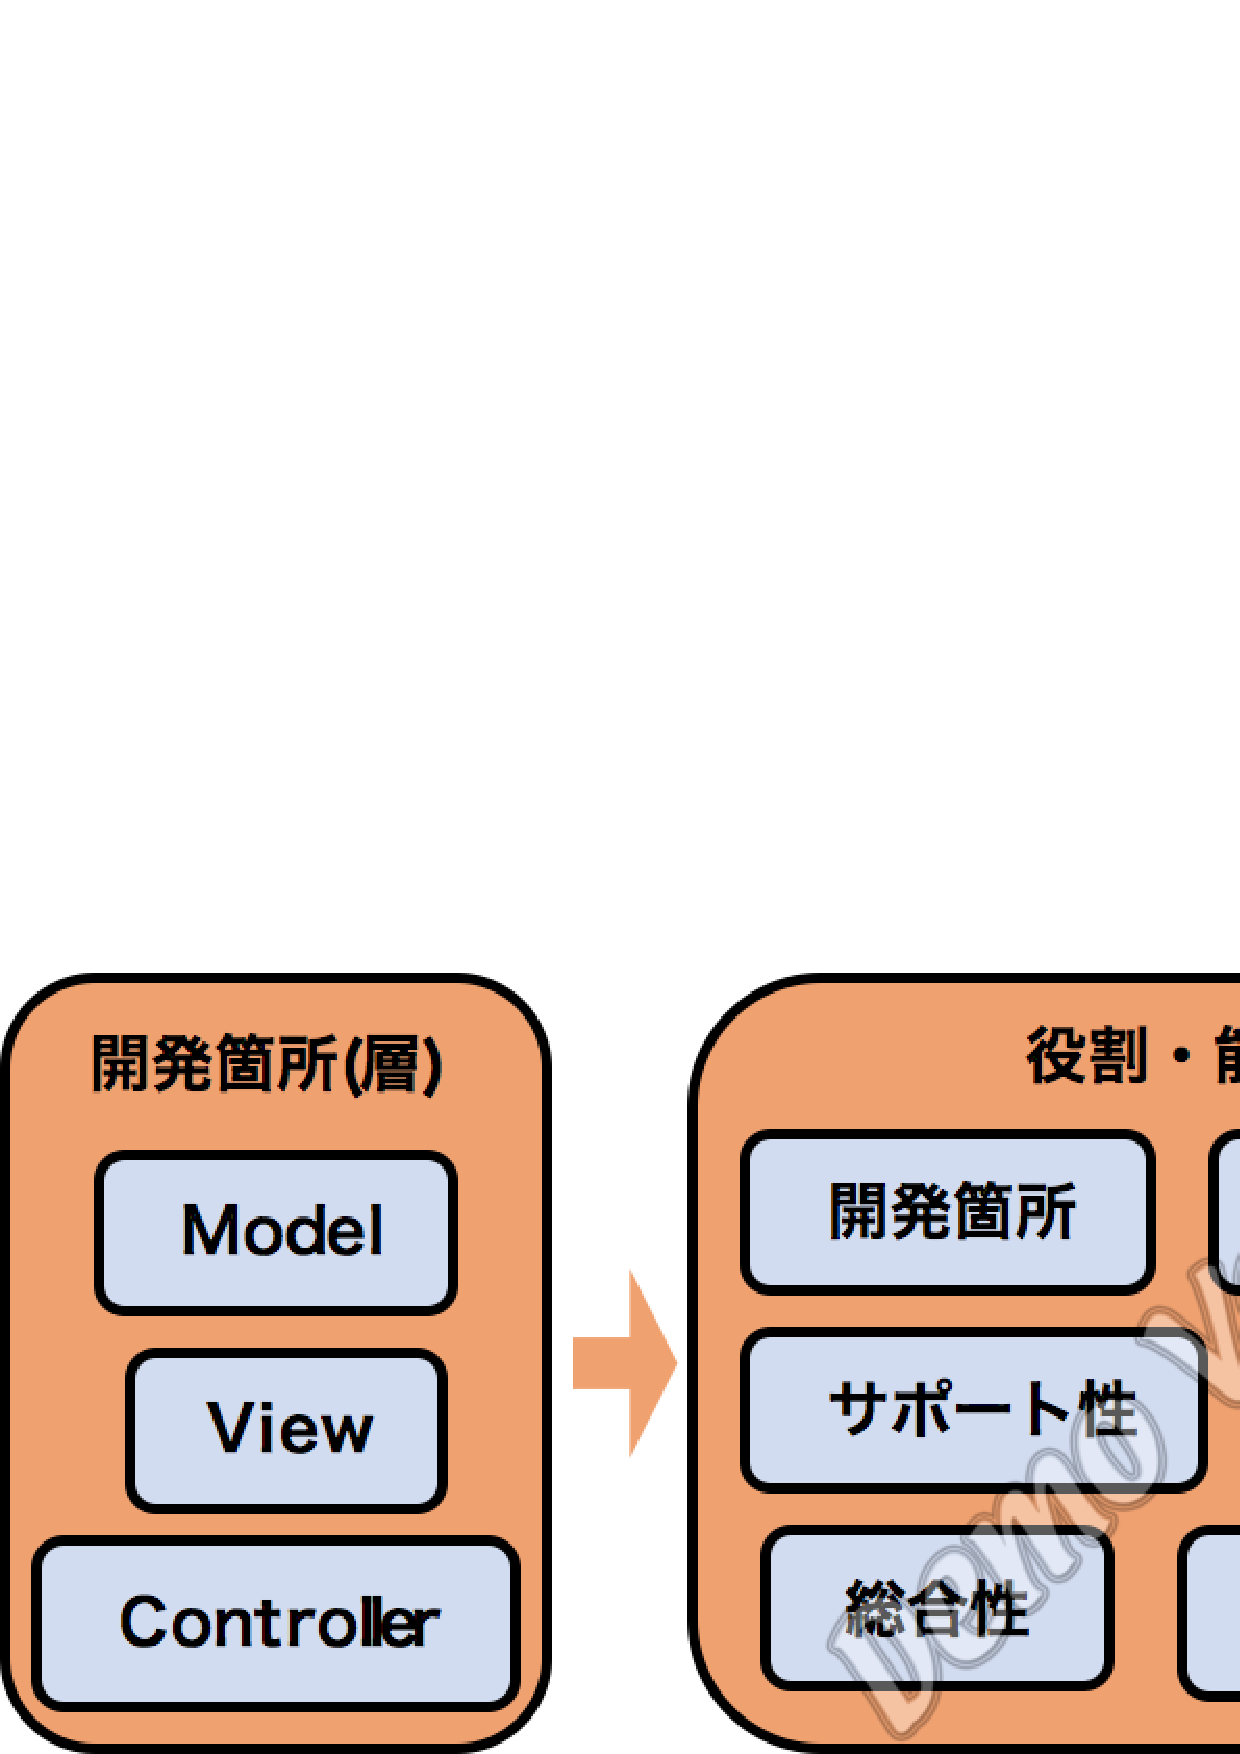
\includegraphics[clip,width=16cm,height=5cm]{figures/overview.pdf}
  \caption{本研究で用いる特徴抽出手法の概要}    \label{sample}
\end{figure}

\subsection{開発箇所(層)の抽出}

MVCフレームワークを対象として,ビュー,モデル,コントロールの各開発層の作成・修正ファイル数に着目することで役割を抽出する(図5.2).例えば,コンロトール層の開発が多い開発者は,フロントエンドエンジニアの役割,モデル層の場合はデータベースエンジニアの役割を担っていると考えられる.なお次節以降の算出方法は,この開発箇所ごとによる作成・修正ファイル数に適用される.
\begin{figure}[!t]
\centering  % 図を真ん中に配置
\includegraphics[clip,width=12cm,height=4cm]{figures/role.pdf}
  \caption{役割の抽出フロー}    \label{sample}
\end{figure}

\subsection{貢献度の抽出}

開発者の貢献度は,質的な貢献度と量的な貢献度に分けて抽出する.
\subsubsection{質的な貢献度}
質的な貢献度は,開発層における重要なモジュール群の開発量に応じて算出する(図5.3).例えば,他の関数からの参照回数が多いライブラリ関数を開発している開発者は,質的な貢献度が高いと考えられる.そこで,参照回数の大い関数の作成数bがしきい値βより大きい場合,そのライブラリ関数の開発者はプロジェクトの質的な貢献度が高いと判定する(表5.1).
\begin{figure}[!t]
\centering  % 図を真ん中に配置
\includegraphics[clip,width=16cm,height=3cm]{figures/contribution_quality.pdf}
  \caption{質的な貢献度の抽出フロー}    \label{sample}
\end{figure}

\begin{table}[htb]
  \begin{center}
    \begin{tabular}{|c||c|} \hline
      cの範囲 & 貢献値  \\ \hline
      0<b≦β1 & 1 \\ \hline 
      β1<b≦β2 & 2 \\ \hline 
      β2<b≦100 & 3  \\ \hline
    \end{tabular}
  \end{center}
  \caption{質的な貢献度のレベル}    \label{sample}
\end{table}

\subsubsection{量的な貢献度}
量的な貢献度は,開発者が作成・修正したソース・ファイル数に応じて算出する.ビュー,モデル,コントロールの各層において,新規作成したソース・プログラムおよび他者開発ソース・プログラムを修正した割合cに応じて,量的な貢献度を算出する(表5.2).
\begin{table}[htb]
  \begin{center}
    \begin{tabular}{|c||c|} \hline
      cの範囲 & 貢献値  \\ \hline
      0<c≦γ1 & 1 \\ \hline 
      γ1<c≦γ2 & 2 \\ \hline 
      γ2<c≦100 & 3  \\ \hline
    \end{tabular}
  \end{center}
  \caption{量的な貢献度のレベル}    \label{sample}
\end{table}

\subsection{サポート性の抽出}

サポート性は,他の開発者への援助の度合いを表す性質であり,他者開発ソース・プログラムのうち,修正したソース・プログラムから算出する.他者開発ファイルの修正数がしきい値δ以上の際に,その開発者はサポート性があるとする.

\subsection{先導性の抽出}

各開発層における新規ファイルの作成数や,設定ファイル,ライブラリ定義ファイル等,システム環境構築に必要なファイルや・プログラムを率先して作成することは,プロジェクトに参加する他の開発者が効率よく開発進める上で重要である.このため,システム開発に必要なファイルやプログラムのコミット数が多い開発者は,先導性が高いと判定する.

\subsection{総合性の抽出}

総合性は,前節で述べたような,各開発層の視点に基づいた貢献性,サポート性,先導性の複合条件によって決定する.条件は対象となるプロジェクトによって異なるが,例えばサポート性と先導性があることを条件とすれば,この2つの性質を同時に満たす開発者にリーダー性があると判定する.
%--------------------------------------------------------------------
\chapter{実験と結果}
5章で述べた特徴抽出手法をGitHub上のプロジェクトを対象とした実験を行う.そこで本章では,実験の準備やその対象,実験の方法,そして実験の結果について述べる.
\section{実験準備}
(※備忘録)1月12日までにこの章の結果の表や文章をを入れていく
\\本節では,実験対象プロジェクトや実験方法といったような,実験を行う上で必要となる準備に関して述べる.
\subsection{実験対象プロジェクト}
GitHubAPIを用いて,Ruby on Rails言語を利用しているプロジェクトを取得した.
実験の対象となるのは以下のプロジェクト.
\\〜〜〜表をいれる〜〜〜〜〜
\\octopub
\\where2help
\\trusty-cms
\\poly
\\yacs
\\coderdojoljp
\\hackweek
\\それぞれプロジェクトP1〜P7とする.

\subsection{実験方法}

それぞれのプロジェクトのしきい値は〜とする.総合性は合計値が〜のときに......とした.
\section{実験結果}
表6.1〜表6....に結果を示す
\subsection{プロジェクトP1}

〜〜〜〜〜〜〜表6.1をはる〜〜〜〜〜〜〜
\subsection{プロジェクトP2}

〜〜〜〜〜〜〜表6.2をはる〜〜〜〜〜〜〜

\chapter{考察}

\section{対象}
実実験したプロジェクトの,(全てor考察がしやすいやつをピックアップ)したものを考察対象とする
\section{考察結果}

ここがこうなっているから,この開発者は〜だと言える.
%--------------------------------------------------------------------

%--------------------------------------------------------------------
\chapter{結論と今後の展望}

\section{まとめ}

Java言語との比較では,惨敗であり,FUNは2倍の
記述量を必要とした.しかし,これは,Javaのもつ
パッケージIKURAが非常に強力であるためで,
同一機能をもつライブラリを用意することにより,
FUNにも同様の能力を持たせることができることが判明した.

\section{今後の展望}

Java言語との比較では,惨敗であり,FUNは2倍の
記述量を必要とした.しかし,これは,Javaのもつ
パッケージIKURAが非常に強力であるためで,
同一機能をもつライブラリを用意することにより,
FUNにも同様の能力を持たせることができることが判明した.


%--------------------------------------------------------------------
%--------------------------------------------------------------------
\chapter*{謝辞}

本研究において、長期にわたる評価実験に協力いただきました、株式会社○○の△△△△様に感謝いたします.


%--------------------------------------------------------------------
% 参考文献
\begin{thebibliography}{20}
 \bibitem {GitHub} GitHub.
 \bibitem {Onoue_English} Onoue, S., Hata, H. and Matsumoto,K.: A Study of the Characteristics of Developers Activities in Github, Proc.IWESEP ’13, pp.7–12 (2013).
 \bibitem{GitHub_API} GitHub API.
 \bibitem{Characteristic}Exploring Expressions of Emotions in GitHub Commit Messages,
\\ http://geeksta.net/geeklog/exploring-expressions-emotions-github-commit-messages/
 \bibitem{Matsubara} 松原 克弥,伊藤 恵,木塚 あゆみ,コード管理ツールGitを活用した分散PBLにおけるチーム活動過程の可視化の試み, 2016.
 \bibitem{Onoue_Japan} 尾上 紗野, 畑 秀明, 松本健一, GitHub上の活動履歴分析による開発者分類, 情報処理学会論文誌, Vol.56-2-715-719, 2015.
 \bibitem{risyo}李書, 鷹野 孝典,分散バージョン管理システムの共同開発履歴に基づいた開発者の特徴抽出手法の検討,情報処理学会研究報告,2015-162-1(1), pp.1-8, 2015.
\end{thebibliography}


% 以降,付録(付属資料)であることを示す
\appendix

%--------------------------------------------------------------------
\chapter*{付録その1} % \chapter{}を使うと「付録A ***」となる

付録その1(プログラムのソースリストなど)を必要があれば載せる

%--------------------------------------------------------------------
\chapter*{付録その2}

付録その2(関連資料など)を必要があれば載せる

%--------------------------------------------------------------------
% 図一覧
\listoffigures

%--------------------------------------------------------------------
% 表一覧
\listoftables

\end{document}
